\begin{table*}[t]
\renewcommand{\arraystretch}{1.05}
 \caption{Performance comparison on our FlyTracing test blocks.}
  \centering
  \begin{tabular}{|l|c@{\hspace{7pt}}c@{\hspace{8pt}}c|c@{\hspace{8pt}}c@{\hspace{8pt}}c|c@{\hspace{8pt}}c@{\hspace{8pt}}c|c@{\hspace{8pt}}c@{\hspace{8pt}}c|}
    \hline
    Dataset & \multicolumn{3}{c|}{Avg. on 3K test blocks} & \multicolumn{3}{c|}{Misalignment }& \multicolumn{3}{c|}{Missing sections } & \multicolumn{3}{c|}{Mixed degradation}\\
    \hline
    Method   & Rec. & Prec. & F1 & Rec. & Prec. & F1 & Rec. & Prec. & F1 & Rec. & Prec. & F1\\
    \hline
    Connect-Embed o. &  $0.890$ & $0.926$ & $0.908$ & $0.738$ & $0.886$ & $0.805$ & $0.890$ & $0.937$ & $0.914$ & $0.810$ & $0.907$ & $0.856$\\
    \hline
    EdgeNetwork  & $0.859$ & $0.969$ & $0.911$ & $0.626$ & $0.944$ & $0.752$& $0.690$ & $0.958$ & $0.802$& $0.699$ & $0.960$ & $0.809$\\
    + Intensity & $0.881$ & $0.970$ & $0.923$ & $0.658$ & $0.946$ & $0.776$& $0.748$ & $0.952$ & $0.838$& $0.713$ & $0.960$ & $0.818$ \\
    + Seg-Embed & $0.870$ & $0.969$ & $0.916$& $0.668$ & $0.937$ & $0.782$& $0.766$ & $0.945$ & $0.846$& $0.749$ & $0.955$ & $0.840$\\
    + Connect-Embed & $0.883$ & $0.971$ & $0.925$& $0.673$ & $0.937$ & $0.783$& $0.748$ & $0.960$ & $0.841$& $0.743$ & $0.962$ & $0.839$\\
    \hline
    PointNet++  & $0.847$ & $0.939$ & $0.891$& $0.628$ & $0.893$ & $0.737$ & $0.693$ & $0.895$ & $0.781$& $0.672$ & $0.903$ & $0.771$\\
    + Intensity  & $0.865$ & $0.949$ & $0.905$ & $ 0.646$ & $0.911$ & $0.756$ & $0.767$ & $0.892$ & $0.825$ & $0.748$ & $0.914$ & $0.823$\\
    + Seg-Embed & $0.914$ & $0.954$ & $0.934$ & $0.739$ & $0.930$ & $0.824$& $0.812$ & $0.924$ & $0.864$& $0.816$ & $0.914$ & $0.862$\\
    + Connect-Embed & $\mathbf{0.932}$ & $\mathbf{0.972}$ & $\mathbf{0.952}$& $\mathbf{0.834}$ & $0.941$ & $\mathbf{0.884}$ & $\mathbf{0.909}$ & $\mathbf{0.963}$ & $\mathbf{0.935}$ & $\mathbf{0.883}$ & $0.949$ & $\mathbf{0.915}$\\
    
    \hline
  \end{tabular}
  \label{over-all}
\end{table*}

\section{Experiments and Results}
\label{Experiment}
 
\subsubsection{Model Configurations.} 
Our EmbedNet follows the architecture of residual symmetric U-Net~\cite{lee2017superhuman}, which tackles anisotropic serial-sectioning EM images with mixed 2D and 3D convolutional layers. We add a Squeeze-and-Excitation block~\cite{hu2018squeeze} to each scale to enhance the embedding expression capability. We set the input volume size as $129 \times 129 \times 17$ under the voxel resolution of $16\times16\times40 nm^3$, and the embedding dimension $k=16$. 
%
The EdgeNetwork~\cite{matejek2019biologically} employs a 3DCNN composed of three convolutional layers with filter sizes 16, 32, and 64, respectively, taking a cube with a side length of $1200nm$ and resized to $52\times52\times18$ as the input. The point clouds are sampled within a cube in size of $2560nm$, and down-sampled to $2048$ points by FPS.  
 

\subsubsection{Training Details.}
We train the embedding network with AdamW optimizer for $500k$ iterations with a batch size of $8$, and apply data augmentation including random rotation, rescale, flip, and grayscale intensity augmentation. The initial learning rate is set to $0.002$ with warmup and a step decay scheduler. 
The number of negative sample pairs $n=20$. 
%
To enhance the learning from EM images with section missing and misalignment, we further fine-tune our EmbedNet on a subset of training blocks where the embedding network has a higher loss at the first round of training.  

The EdgeNetworks (with and without image embedding features) are trained with AdamW optimizer for $45k$ steps with a batch size of $128$. The PointNet++ models are trained with AdamW optimizer for $200k$ steps with a batch size of $92$. 
Because in real neuron tracing scenarios, there are much more adjacent segment pairs that do not belong to the same neuron, we train our connectivity prediction network with more negative segment pairs by setting the ratio between positive samples and negative samples to $3:7$. 
All the $422k$ positive segment pairs in the 1000 training data blocks are included during training and validation.  


\subsection{Results of Segment Connectivity Prediction}

\subsubsection{Metrics.} 
To evaluate the segment connectivity prediction performance, we use the recall and precision metrics. On the $3000$ testing blocks, all the $1,178k$ positive segment pairs are used for evaluation. For each positive pair, we pick one segment as the query segment of the pair and randomly sample one of its neighboring segments from another neuron near the truncation point to form a negative pair. 
Two segments $S_a, S_b$ are determined as connected as the same neuron if $f(S_a,S_b)>0.5$.

\subsubsection{Comparison of Multiple Methods.}
We evaluate various combinations of image and morphology representations and report the results in Table~\ref{over-all}.
For the image features, we also evaluate `Intensity' and `Seg-Embed'. `Intensity' corresponds to the raw voxel intensity of the EM image, while `Seg-Embed' refers to the image embedding approach for neuron segmentation proposed in \cite{lee2021learning}. 
In our experiment, the `Seg-Embed' embedding is trained using dense neuron segmentation annotation from the CREMI dataset, sourced from three sub-volumes of FAFB. Notably, the embedding in \cite{lee2021learning} serves as a surrogate of the affinity map for neuron segmentation, rather than for correcting segmentation split errors. 
Image features are not exploited in the vanilla `EdgeNetwork' or `PointNet++' model.
In addition to these combinations, we also present the prediction performance using single modalities. `Connect-Embed o.' denotes that we determine $f(S_a,S_b)=1$ if the distance between the mean embedding of the two segments $\left\|\bm{\mu}_{query}-\bm{\mu}_{candidate}\right\|<\delta_d$. 

\begin{figure}[t]
    \centering
    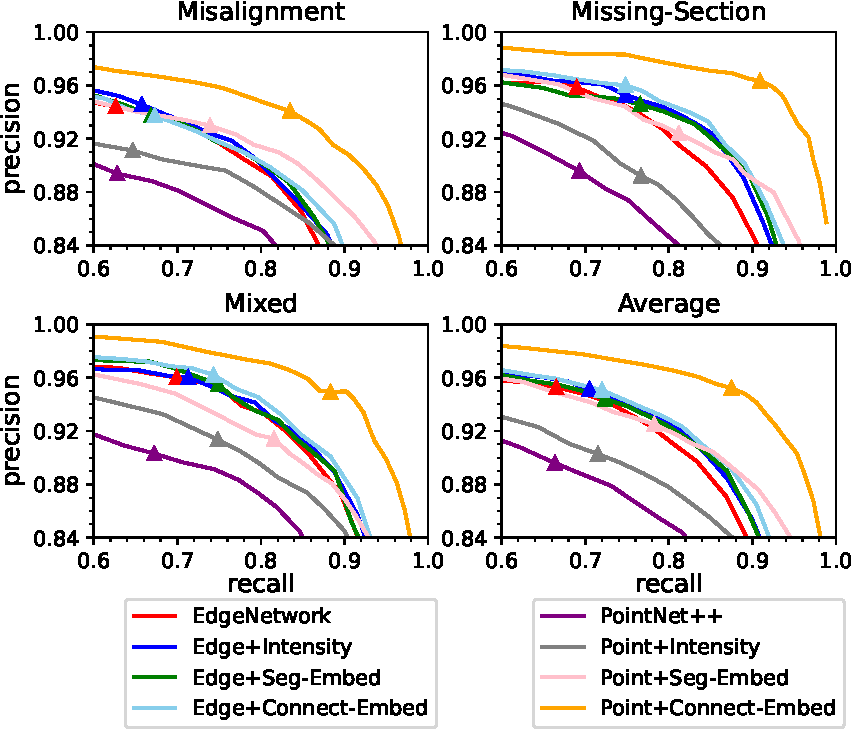
\includegraphics[width=0.45\textwidth]{figs/thresh.pdf}
    \caption{Precision-recall curves of different models on challenging blocks with image degradation. The triangle markers denote the performance using threshold $f(S_a,S_b)>0.5$. } 
    \label{thresh}
\end{figure}

As Table~\ref{over-all} shows, the combination of point cloud representation and our connectivity-aware embedding ``+Connect-Embed' performs the best. 
Compared with 3D voxel-based model EdgeNetwork, PointNet++ reaps greater advantages from incorporating image features. 
Since 3DCNNs suffer cubical computation increases when enlarging the input volume size, the EdgeNetworks have to consider the trade-off between input resolution and field of view, preventing them from getting the advantages of local fine-grained image features and global morphological features simultaneously. 
On the contrary, our proposed fusion of point cloud with image embedding effectively preserves local sophisticated image characteristics, while encompassing morphology information across a broad field of view within a fixed number of input points. 
%
In addition, among the three manners of image feature encoding, including intensity only, segmentation-based embedding, and our connectivity-aware embedding, our embedding is the most effective for segment connectivity prediction. % 


Particularly for the EM volume blocks that suffer from severe image degradations, such as misalignment or section missing, the proposed PointNet++ (+Connect-Embed) yields remarkable enhancements to competitors. 
Among the $3,000$ test blocks, we select $10$ blocks containing $300\!\sim\!800nm$ misalignment, $10$ blocks containing $2\!\sim\!3$ missing sections, and $5$ blocks suffering from both degradations (typically one section missing followed by misalignment of $200\!\sim\!300nm$). 
%
Fig.~\ref{thresh} depicts the precision-recall curves of the models on the low-quality EM blocks.
Notably, the curve of our proposed feature combination consistently outperforms the others by a substantial margin.
This significant improvement is mainly brought by the proposed embeddings that can compensate for the information loss of segment morphology at the regions with image degradation and shape distortion. The raw voxel intensity retains only sparse low-level information from the image when combined with the point cloud, therefore providing limited improvement. On the other hand, without the supervision of pair-wise contrast of segments throughout the brain, Seg-Embed \cite{lee2021learning} fails to generate robust embeddings against imaging artifacts. In contrast, our embedding approach provides both structural and fine-grained image features.

\begin{figure}[t]
    \centering
    \includegraphics[width=0.48\textwidth]{figs/improvement.pdf}
    \caption{Visualization of several segment pairs whose connection relations are correctly predicted by model PointNet++ with `Connect-Embed'. In the two lower rows, we show the representative EM image sections and corresponding embeddings of the samples in the color boxes. }
    \label{visual}
\end{figure}

\subsubsection{Embedding Visualization.}
 %
 In Fig.~\ref{visual}, we show two sets of segment pairs whose connection relationships are correctly classified by our PointNet++ with `Connect-Embed' model. 
We visualize the embeddings using PCA to project the high-dimensional embedding vector onto the RGB color space. 
Without the image embedding, the PointNet++ model fails to predict the connectivity of these segment pairs because of the ambiguous morphology. The positive pairs are often subject to image degradation, resulting in morphological distortions or too small segments without sufficient evidence for connection. 
On the other hand, the morphology of misclassified negative pairs is hard to distinguish from positive connectivity pairs. 
In contrast, our embedding provides distinctive clues for neuron tracing, effectively complementing the distorted morphological features. Despite the variations in the location and appearance of the neurons across sections, our embedding remains discriminative and consistent. 

\subsubsection{Ablation Study of EmbedNet.}
We measure the discriminative ability of EmbedNet under different loss configurations. The discriminative ability is defined as the rank of $\left\|\bm{\mu}_{query}\!-\!\bm{\mu}_{pos}\right\|$ among all $n+1$ candidates $\{\!\left\|\bm{\mu}_{query}\!-\!\bm{\mu}_{pos}\right\|\!,\left\|\bm{\mu}_{query}\!-\!\bm{\mu}_{neg}^1\right\|\!,...,\left\|\bm{\mu}_{query}\!-\!\bm{\mu}_{neg}^n\right\|\!\}$. 
We report the mean rank on $3$ test blocks. The adaptive weighting strategy performs the best since $L_{seg}$ gives dense supervision of voxel-wise segmentation in earlier steps, while decreasing the weight enforces the model to focus on learning discriminative features from pairwise connection annotations, i.e., $L_{split}$ and $L_{merge}$, in later steps.


\begin{table}[t] 
\setlength\tabcolsep{6pt}
\centering
\caption{Discriminative ability (the lower the better) of the embedding network with different weights of $L_{seg}$ ($\lambda_3$), where $\infty$ indicates that the model is trained with $L_{seg}$ only, and `Adaptive' denotes the decreasing strategy of $\lambda_3$. }
\label{ablation}
\begin{tabular}{l|ccc|c}
\hline
$\lambda_3$ & Block A & Block B & Block C & Average \\
 \hline
$\infty$ & $4.49$ & $4.18$ & $3.52$ & $4.07$ \\
$1$ & $2.46$ & $2.14$ & $1.85$ & $2.15$ \\
$0.1$ & $1.73$ & $1.60$ & $1.36$ & $1.57$ \\
$0$ & $2.34$ & $2.07$ & $2.04$ &$2.15$ \\
\hline
Adaptive & $\mathbf{1.59}$ & $\mathbf{1.45}$ & $\mathbf{1.19}$ & $\mathbf{1.41}$ \\
\hline
\end{tabular}
\end{table}
 
\subsubsection{Tracing Result on FAFB Mushroom Body.}
We also evaluate our proposed model PointNet++ with the `Connect-Embed ' within a real tracing scenario on the FAFB dataset. Following the evaluation setting described in \cite{fafb-ffn}, we evaluate the segmentation with a set of 166 ground truth neuronal skeletons produced by human tracers \cite{FAFB} using modified expected run length (ERL) metric from \cite{wei2021axonem}. 
We crop a volume of size $64\times44\times56$ $\mu m^3$ from the mushroom body region which contains around $10\%$ of the ground truth skeleton nodes and exclude the subvolumes in the training set. The candidate pairs and truncated points are estimated from the endpoints of segment skeletons as \cite{matejek2019biologically}. Using FAFB-FFN1 as the initial EM image segmentation, with a merging threshold of $0.98$, our automatic proofreading with pairwise segment connectivity prediction increases ERL by $28.8\mu m$ (a relative increase of $8.1\%$ ). 